\section{Grundlagen}
Das folgende Kapitel stellt die theoretischen und technologischen Grundlagen vor, die für das Verständnis und die Umsetzung dieser Arbeit erforderlich sind.
Es beginnt mit einer Einführung in die Industrie 4.0, und vermittelt ein grundlegendes Verständnis für das Konzept des digitalen Zwillings.
Anschließend werden die Struktur und Funktion der \acs{aas} sowie die Rolle des digitalen Produktpasses erläutert.
Den Abschluss bilden die technologischen Voraussetzungen für die praktische Umsetzung, darunter beispielsweise die Open-Source-Plattform Eclipse BaSyx und der Kommunikationsstandard OPC UA.
\subsection{Industrie 4.0}
% Nach der dritten industriellen Revolution, die vor allem durch den Einsatz elektronischer Systeme sowie der Informations -und Kommunikationstechnologie zur Automatisierung gekennzeichnet ist, vollzieht sich aktuell ein neuer technologischer Wandel, die vierte industrielle Revolution.
% Besser bekannt als Industrie 4.0, beschreibt sie die umfassende Vernetzung und Integration der physischen mit der digitalen Welt durch den Einsatz Cyber-physischer Systeme.

Der Begriff Industrie 4.0 wurde erstmals im Jahr 2011 im Rahmen eines von der deutschen Bundesregierung initiierten Zukunftsprojekts eingeführt, das auf die Förderung der Informatisierung in der industriellen Fertigung/Produktion abzielt.
Angestrebt wird eine Stärkung der Wettbewerbsfähigkeit der deutschen Industrie sowie eine Verbesserung der Marktposition deutscher Unternehmen im globalen Wettbewerb.
Industrie 4.0 steht dabei für die vierte industrielle Revolution und beschreibt die umfassende digitale Transformation industrieller Wertschöpfungsprozesse. 
Im Zentrum steht die intelligente Vernetzung von Menschen, Maschinen und Produkten über moderne digitale Kommunikationsnetzwerke, durch die eine weitreichende Integration der physischen mit der digitalen Welt ermöglicht wird.

Zur besseren Einordnung von Industrie 4.0 ist ein Blick auf die vorangegangenen industriellen Revolutionen hilfreich.
Die Industrialisierung begann bereits Mitte des 18. Jahrhunderts in Großbritannien und breitete sich von dort an weltweit aus. 
Mit der Entwicklung der ersten Dampfmaschine setzte die erste industrielle Revolution ein. 
Sie ermöglichte erstmals die Mechanisierung der Fertigung durch den Einsatz von Arbeits- und Kraftmaschinen. 
Dadurch konnten manuelle Tätigkeiten zunehmend durch Maschinenkraft ersetzt werden - insbesondere in der Textil-, Eisen- und Stahlindustrie, die zu den ersten Branchen gehörten, die von dieser Entwicklung profitierten.
Die zweite industrielle Revolution setzte gegen Ende des 19. Jahrhunderts ein und war maßgeblich durch den flächendeckenden Einsatz von Elektrizität geprägt. 
Mit der Erfindung elektrischer Antriebe und des Verbrennungsmotors konnten Maschinen nun auch dezentral betrieben werden - sie waren nicht länger auf zentrale Kraftquellen wie Dampfmaschinen angewiesen. 
Dies ermöglichte eine flexiblere Gestaltung von Produktionsstätten und führte zur Entwicklung einer arbeitsteiligen Massenproduktion mithilfe von Fließ- und Förderbändern.
Ausgehend von dem deutschen Wirtschaftswunder in den sechziger Jahren des 20. Jahrhunderts entstand in den folgenden Jahrzehnten die dritte industrielle Revolution.
Diese zeichnet sich vor allem durch den Einsatz elektronischer Systeme sowie der Informations- und Kommunikationstechnologie zur Automatisierung aus und ist noch bis heute wirksam.

Aufbauend auf den vorangegangenen industriellen Revolutionen strebt die vierte industrielle Revolution eine tiefgreifende Transformation industrieller Produktionsprozesse an. 
Im Fokus steht dabei die Vernetzung von Systemen, die über moderne Internettechnologien miteinander kommunizieren.
Ziel dieser Entwicklung ist es, die industrielle Wertschöpfung flexibler und effizienter zu gestalten sowie eine stärkere Individualisierung von Produkten zu ermöglichen. 
\cite{Industrie4.0ProduktionAutomatisierung}\cite{EinführungundUmsetzungI4.0}

Trotz der weiten Verbreitung des Begriffs Industrie 4.0 mangelt es in der Literatur und Forschung an einer einheitlichen Definition.
Vor diesem Hintergrund nimmt insbesondere die Plattform Industrie 4.0 \cite{plattform_i40} eine zentrale Rolle in Deutschland ein. 
Dabei handelt es sich um eine gemeinsame Initiative des Bundesministeriums für Wirtschaft und Energie, des Bundesministerium für Forschung, Technologie und Raumfahrt sowie führender Industrieverbände (z.B. VDMA, Bitkom, ZVEI), Unternehmen, Forschungseinrichtungen und Gewerkschaften.

Die Plattform ist maßgeblich an der inhaltlichen und strategischen Ausarbeitung der Industrie 4.0 beteiligt und leistet einen entscheidenden Beitrag zur Begriffsdefinition. 
Sie definiert Industrie 4.0 als
\glqq die vierte industrielle Revolution, einer neuen Stufe der Organisation und Steuerung der gesamten Wertschöpfungskette über den Lebenszyklus von Produkten.
Dieser Zyklus orientiert sich an den zunehmend individualisierten Kundenwünschen und erstreckt sich von der Idee, dem Auftrag über die Entwicklung und Fertigung, die Auslieferung eines Produkts an den Endkunden bis hin zum Recycling, einschließlich der damit verbundenen Dienstleistungen.
Basis ist die Verfügbarkeit aller relevanten Informationen in Echtzeit durch Vernetzung aller an der Wertschöpfung beteiligten Instanzen sowie die Fähigkeit aus den Daten den zu jedem Zeitpunkt optimalen Wertschöpfungsfluss abzuleiten. 
Durch die Verbindung von Menschen, Objekten und Systemen entstehen dynamische, echtzeitoptimierte und selbst organisierende, unternehmensübergreifende Wertschöpfungsnetzwerke, die sich nach unterschiedlichen Kriterien wie beispielsweise Kosten, Verfügbarkeit und Ressourcenverbrauch optimieren lassen \grqq~\cite[S. 8]{plattform_i40_definition}.
Diese Definition legt den Fokus auf die durchgängige Digitalisierung und Vernetzung entlang der gesamten Wertschöpfungskette. 
Sie umfasst nicht nur technologische Konzepte wie Echtzeitfähigkeit, autonome Steuerung und selbstorganisierende Systeme, sondern impliziert auch tiefgreifende organisatorische Veränderungen über Unternehmensgrenzen hinweg. 
Dadurch lassen sich nicht nur Qualität, Effizienz und Transparenz entlang des gesamten Produktlebenszyklus deutlich steigern, sondern auch Ressourcenverbrauch, Produktionskosten und Energieeinsatz signifikant reduzieren. 
Industrie 4.0 trägt somit nicht nur zur Verbesserung der Wirtschaftlichkeit bei, sondern leistet auch einen wichtigen Beitrag zur ökologischen Nachhaltigkeit.
% Obwohl Industrie 4.0 häufig als neuartiges Konzept dargestellt wird, basiert es im Kern auf Ideen, die schon seit mehreren Jahrzenten exisiteren.
% Bereits seit den 1980er-Jahren wurden mit Ansätzen wie dem Computer Integrated Manufacturing (CIM) oder der intelligenten Fabrik (Smart Factory) Strategien entwickelt, die auf eine computerintegrierte und automatisierte Produktion abzielen und dabei den Menschen mehr in den Hintergrund rücken.
% Allerdings scheiterten diese frühen Ansätze oft an den technische Möglichkeiten der damaligen Zeit, vor allem fehlte die Infrastruktur, Rechenleistung und Vernetzung.
% Erst mit dem technologischen Fortschritt, insbesondere der Einführung des Internetprotokolls V6 im Jahr 2012, wurde die Grundlage für eine globale, skalierbare Vernetzung von Maschinen, Produkten und Menschen im Sinne des Internet of Things geschaffen.
% Dies ermöglichte erstmals die Realisierung des Internet der Dinge (Internet of Things (IoT)), welches die technologische Basis für die Industrie 4.0 bildet.



\subsubsection{Künstliche Intelligenz}
\subsubsection{RAMI 4.0}
Das \ac{rami} ist ein Leitfaden für die Industrie und dient als Hilfestellung um die digitale Transformation in einem Unternehmen systematisch umzusetzten.
Es wird in der DIN SPEC 91345 \cite{RAMI4.0} standardisiert und soll helfen, die komplexen Anforderungen an die Industrie 4.0 für die Allgemeinheit verständlich zu machen.
Das Modell unterteilt sich in drei verschiedene Schichten wie in Abbildung xy zu sehen.

\begin{figure}[htbp]
    \centering
    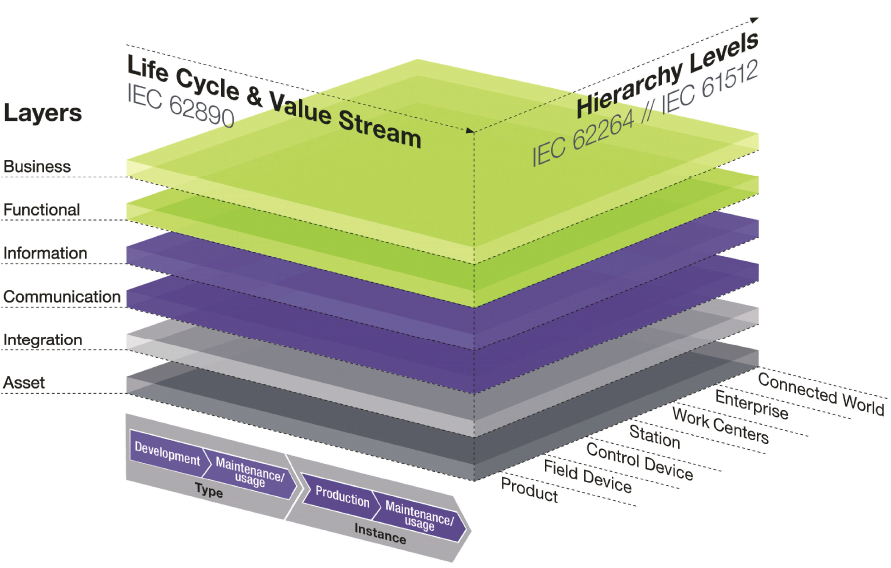
\includegraphics[width=1\textwidth]{Bilder/RAMI.PNG}
    \caption{Referenzarchitekturmodell Industrie 4.0 (RAMI 4.0)}
    \label{fig:klassifizierungDT}
\end{figure}

\newpage
\subsection{Digitaler Zwilling}
Digitale Zwillinge gelten als eine der Schlüsseltechnologien der Industrie 4.0.
Als digitales Gegenstück eines physischen Objekts - sei es eine Maschine ein Produkt oder eine komplette Anlage - bilden sie dessen Zustand, Verhalten und Leistung virtuell ab.
Dadurch ermöglichen sie eine konsistenete Erfassung von Daten, das Simulieren von Prozessen und das frühzeitige Erkennen von Optimierungspotenzialen.

Das Konzept selbst wurde erstmals von Michael Grieves im Jahr 2003 in einer Präsentation zum Product Lifecycle Management vorgestellt. 
Grieves definierte drei grundlegende Komponenten (vgl. \cite{DTGrieves}) , die zusammen das Informationsmodell des digitalen Zwilling bilden:
\begin{itemize}
    \item ein reales Objekt in der physischen Welt,
    \item ein digitales Abbild dieses Objekts in einem virtuellen Raum, sowie
    \item eine Schnittstelle, die den Informationsfluss zwischen diesen beiden ermöglicht.
\end{itemize}

Auf Basis des von Grieves entwickelten Informationsmodells hat sich der Begriff des digitalen Zwillings kontinuierlich weiterentwickelt.
Aufgrund verschiedener Fachgebiete und inkonsistenter Definitionen haben sich in der Vergangenheit allerdings eine Vielzahl unterschiedlicher Ausprägungen des Begriffs gebildet.
Diese unterscheiden sich insbesondere in der Tiefe der Datenintegration zwischen dem physischen Objekt und seinem virtuellen Abbild.
Während ein einfacher digitaler Zwilling lediglich ein einfaches Modell mit statischen Daten ist, ermöglichen fortgeschrittene Zwillinge einen bidrektionalen Datenaustausch zwischen physischem und virtuellem Objekt. 

Für ein besseres Verständnis und zur tieferen Klassifizierung ist es zunächst hilfreich, zwischen Typen und Instanzen des digitalen Zwillings zu unterscheiden.
Typen sind allgemeine Abbilder, die grundlegende Eigenschaften und Verhaltensmodelle einer Produktgruppe beschreiben. 
Sie können mit einer Klasse in der Softwarentwicklung verglichen werden, die als Vorlage für konkrete Instanzen dienen.
Typen können zum Beispiel einen bestimmten Maschinentyp hinsichtlich Aufbau, Stuktur oder Schnittstellen beschreiben, ohne dabei Bezug zu einer einzelnen physischen Maschine zu nehmen.
Instanzen wiederrum sind einzigartig, und beschreiben ein konkretes Produkt, wie zum Beispiel eine Maschine, die einzigartig über eine Seriennummer identifizierbar ist.
Häufig sind Instanzen Aussprägungen eines Types mit einer Verbindung zu einem realen Objekt, wodurch beispielsweise die Überwachung des Zustands einer Maschine ermöglicht wird.
Analog zur Softwarentwicklung können diese als instanziiertes Objekt einer Klasse gesehen werden. \cite{ZEISS}

Je nach Art des Informationsflusses sowie dem Grad der Ausprägung der Verbindung zur realen Welt werden Instanzen digitaler Zwillinge häufig in drei Kategorien klassifiziert: das digitale Modell, den digitalen Schatten und den digitalen Zwilling \cite{ClassificationDT}.
Obwohl diese Begriffe im allgemeinen Sprachgebrauch oft synonym verwendet werden, unterscheiden sie sich deutlich hinsichtlich ihrer Funktion und Kopplung zum realen Objekt.
Digitale Modelle sind statische Abbilder physischer Objekte, haben jedoch keine Verbindung zu diesen. 
Oft werden sie zur Veranschauclichung oder Konstruktion genutzt, wie zum beispiel ein 3D-Modell einer Maschine.
Zwar können reale Daten, wie etwa Maße oder Materialeigenschaften einer Anlage oder Maschine in ein solches Modell integriert werden, allerdings erfolgt die Eingabe dabei immmer manuell.
Änderungen an dem realen Objekt werden nicht automatisch aktualisiert und bleiben somit ohne Einfluss auf das digitale Modell.
Der digitale Schatten ergänzt das digitale Modell um eine unindirektionale Verbindung zum realen Objekt.
Dabei fließen Daten des physischen Objekts meist in Echtzeit über zum Beispiel geeignete Sensoren zum digitalen Objekt.
Der Schatten bildet den aktuellen Zustand des Objekts ab, hat aber keine Rückkoplung zu diesem.
Ein typisches Beispiel für einen digitalen Schatten wäre das Condition Monitoring, wobei der Zustand einer Maschine mit geeigneten Sensoren abgebildet wird.
Mit einer aktiven Rückkoplung zum realen Objekt wird der digitale Schatten zum digitalen Zwilling.
Es entsteht eine Feedback-Schleife und erlaubt dem virtuellen Objekt Einfluss auf das reale System zu nehmen.

% Quelle: file:///C:/Users/Heinke/Documents/Bachelorarbeit/02%20Literatur/Digitaler_Zwilling/Klassifizierung_DT.pdf

\begin{figure}[htbp]
    \centering
    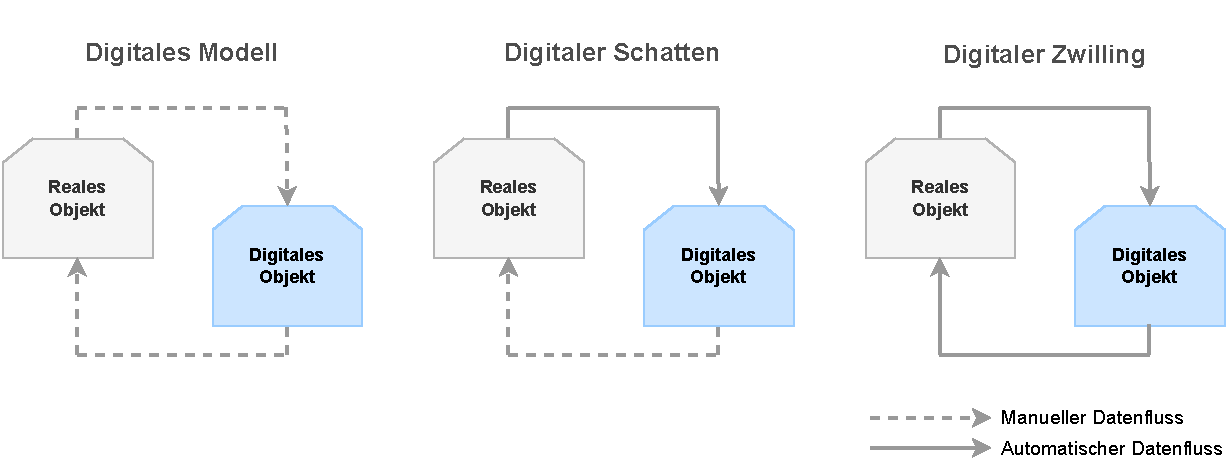
\includegraphics[width=1\textwidth]{Bilder/klassifizierung_DT.pdf}
    \caption{Klassifizierung des DT}
    \label{fig:klassifizierungDT}
\end{figure}

% Digitales Modell, digitaler Schatten und digitaler zwilling
Im industriellen Umfeld werden digitale Zwillinge in vielen unterschiedlichen Bereichen genutzt.
Sie kommen entlang des gesamten Lebenszyklus eines Produkts oder Systems zum Einsatz - von der Entwicklung über die Produktion bis hin zum Betrieb und der Wartung. 
Dabei ist jedoch zu beachten, das in der Praxis häufig auch digital Modelle oder digitale Schatten als digitale Zwillinge bezeichnet werden, obwohl sie technisch gesehen nicht alle Merkmale eines \glqq echten\grqq~digitalen Zwillings aufweisen und somit nicht ihr volles Potenzial entfalten.

Bereits bei der Entwicklung von Produkten können digitale Zwillinge einen erheblichen Vorteil bieten. 
Indem bereits frühzeitig digitale Modelle oder Simulationen eingesetzt werden, entfällt die Notwendigkeit physischer Prototypen, was Entwicklungszeiten und Kosten deutlich senken kann. Während der Produktion ermöglichen sie eine durchgängige Überwachung, Analyse und Optimierung von Fertigungsprozessen durch die Integration von Echtzeitdaten.
Sie unterstützen die virtuelle Inbetriebnahme von Maschinen und dienen als Grundlage für die vorausschauende Wartung (Predictive Maintenance), wodurch Stillstandzeiten einer Maschine reduziert werden können.
Nicht zuletzt dienen digitale Zwillinge als zentrale Datenplattform, in der alle relevanten Informationen aus verschiedenen Datenquellen gebündelt werden.
Sie bilden somit eine konsistente Datenbasis und können beispielsweise bei dem Entwicklungsprozess eines Produktes helfen. \cite{DTForSmartManufacturing}

% Trotz der zahlreichen Vorteile gibt es auch einige Herausforderungen bei der Einführung digitaler Zwillinge in einem Unternehmen.
% Zunächst müssen Daten aus unterschiedlichsten Systemen wie ERP oder MES in ein digitales Modell zusammengefasst werden.
% Häufig liegen diese jedoch in heterogenen Formaten vor, was die Integration erheblich erschwert.


% Darüber hinaus gestaltet sich die Modellierung selbst oft als anspruchsvoll, da sowohl spezielles Fachwissen als auch geeignete Tools zur Modellierung benötigt werden.
% Insbesondere beim Einsatz digitaler Zwillinge über Unternehmensgrenzen hinweg muss ein einheitliches Verständnis der Daten geschaffen werden.
% Uneindeutige Beschreibungen können zu Fehlinterpretationen -und entscheidungen führen.
% Nicht zuletzt stell die Cybersicherheit eine zentrale Herausforderung dar - vor allem wenn cloudbasierte Lösungen oder unternehmensübergreifende Datenräume genutzt werden.

Die Implementierung digitaler Zwillinge erweist sich in der Praxis jedoch oftmals als sehr anspruchsvoll.
Eine zentrale Herausforderung ist die fehlende Interoperabilität zwischen verschiedenen IT-Systemen.
Sowohl innerhalb eines Unternehmens als auch unternehmensübergreifend bilden sich dadurch häufig voneinander isolierte Datenbestände, die nicht systemübergreifend nutzbar sind.
Solche sogenannten Informationssilos können die Umsetzung eines konsistenten digitalen Zwillings erheblich erschweren, da die relevanten Informationen und Daten zunächst aus unterschiedlichen Systemen wie Enterprise Resource Planing (ERP), Manufacturing Execution System (MES) oder Computer Aided Design (CAD) zusammengeführt werden müssen.
Hinzu kommt, das diese Daten oftmals in unterschiedlichen, nicht standardisierten Formaten vorliegen, was eine automatisierte Integration zusätzlich erschwert.
Diese Problematik zeigt sich nicht nur innerhalb einzelner Unterhnehmen, sondern auch entlang der gesamten Wertschöpfungskette, etwa wenn verschiedene Akteure einer Lieferkette heterogene Datenformate und proprietäre Austauschprotokolle verwenden.
Ein digitaler Zwilling, der in einem Unternehmen A erstellt wurde, kann dadurch von einer Anwendung oder einem weitern digitalen Zwilling eines Unternehmens B nicht ohne Weiteres intepretiert oder verwendet werden.
Es ist daher essenziell, digitale Zwillinge in einem interoperablen Format bereitzustellen, um eine einheitliche Interpretation und Nutzung auch über Unternehmensgrenzen hinweg zu ermöglichen.
\cite{DTandAASConceptsInI4.0}


% Definition nach Stark und Damerau des DT: 

% A digital twin is a digital representation of an active unique product (real device, object, machine, service, or intangible asset) or unique product-service system (a system consisting of a product and a related service) that comprises its selected characteristics, properties, conditions, and behaviors by means of models, information, and data within a single or even across multiple life cycle phases.

% \url{https://link.springer.com/referenceworkentry/10.1007/978-3-642-35950-7_16870-1#citeas}

\newpage
\subsection{Asset Administration Shell}
\label{chap:AAS}
Die Asset Administration Shell (AAS) - deutsch Verwaltungsschale - ist eine Schlüsselkomponente innerhalb des Referenzarchitekturmodells der Industrie 4.0 \cite{RAMI4.0} und bildet die Grundlage für die Umsetzung und Entwicklung interoperabler digitaler Zwillinge im industriellen Umfeld.
Sie wurde maßgeblich von der Plattform Industrie 4.0 entwickelt und erstmlas im Jahr 2016 als Teil von RAMI 4.0 vorgestellt.
Seit ihrer Einführung wurde die AAS kontinuierlich weiterenwtickelt und ist mittlerweile in der internationalen Norm IEC 63278-1 \cite{AASIEC63278} standardisiert.
% Darin wird die AAS als "strukturierte, standardisierte digitale Repräsentation eines Assets" definiert.

Seit 2020 wird die Umsetzung und Weiterentwicklung der AAS von der Industrial Digital Twin Association (IDTA) \cite{IDTA} organisiert und gesteuert.
Ziel der IDTA ist es, den digitalen Zwilling auf Basis der AAS zu standardisieren und in Form von Open Source Softwarelösungen in das industrielle Umfeld zu integrieren.
Die AAS wird dabei in mehreren Spezifikationen der IDTA dokumentiert und beschrieben.
Aktuell bildet die AAS Version 3 den neuesten Entwicklungsstand und ist ebenfalls die Basis für diese Arbeit.
% evtl die Quelle wenn gut https://www.zvei.org/themen/start-der-industrial-digital-twin-association-idta

Die AAS repräsentiert ein Asset digital, indem sie alle relevanten Daten, Eigenschaften und Funktionen über den gesamten Lebenszyklus hinweg in strukturierter und standardisierter Form bereitstellt. 
Sie fungiert somit als digitales Gegenstück eines realen Objekts - also als digitaler Zwilling.
Die Informationen sind in sogenannten Submodellen organisiert, die jeweils spezifische Aspekte eines Assets abbilden.
Dabei kann es sich sowohl um physische Assets (z.B. Maschinen, Anlagen) als auch um virtuelle Assets (z.B. Software, Konzepte) handeln. 
Eine AAS ist stets eindeutig einem Asset zugeordnet und global identifizierbar. 
Durch die Kombination eines Assets mit seiner AAS entsteht eine sogenannte Industrie-4.0-Komponente.

% Durch die standardisierte Struktur bildet die Verwaltungsschale die Grundlage für einen einheitlichen Informationsaustausch über System -und Unternehmensgrenzen hinweg.
% Verwaltungsschalen repräsentieren immer genau ein Asset und müssen global eindeutig identifizierbar sein.
% In der Industrie können Assets physische Objekte, wie eine Anlage oder eine Maschine sein oder aber auch virtuelle Elemente wie Software oder eine Idee.
% In RAMI 4.0 wird davon ausgegangen, das Assets immmer einen konkreten Nutzen für ein Unternehmen bzw. eine Organisation bieten.
\vspace{2em}
\begin{figure}[htbp]
    \centering
    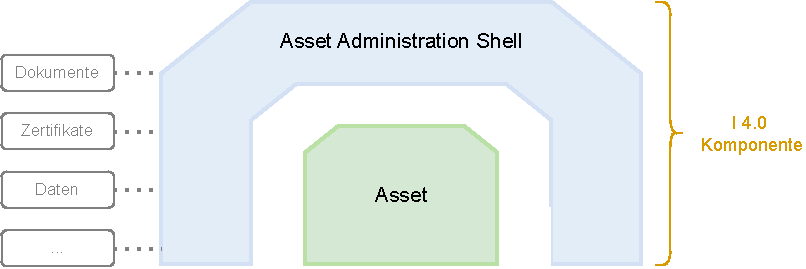
\includegraphics[width=1\textwidth]{Bilder/i4_komponente_neu.pdf}
    \caption{Industrie 4.0 Komponente}
    \label{fig:klassifizierungDT}
\end{figure}

\subsubsection{Aufbau und Struktur}
Allgemein kann zwischen Typ -und Instanz-Verwaltungsschalen unterschieden werden.
Typ-AAS beschreiben allgemeine Eigenschaften eines Produkttypen oder einer Produktlasse wie einen bestimmten Maschinen-Typ, während Instanz-Verwaltungsschalen immer einem spezifischen Objekt zugeordnet werden.
Typen können zum Besipiel allgemeine Dokumente, Eigenschaften oder Merkmale enthalten, die für eine bestimmte Maschinenart gelten.
Sie dienen als standardisierte, wiederverwendbare Vorlage für das Erstellen von Instanzen.
Im Gegensatz dazu werden Instanzen immer einem konkreten physischen Objekt zugewiesen - etwa durch die Seriennummer, den aktuellen Standort oder den Betriebszustand einer Maschine.

Bestimmte Aspekte eines Assets werden gemäß der Spezifikation des Metamodells der AAS \cite{SpezifikationPart1} in verschiedenen Submodellen verwaltet.
Man kann sich dies wie ein Schubladensystem vorstellen, wobei jede Schublade einen bestimmten Bereich des Assets abdeckt - beispielsweise die technischen Stammdaten, das Typenschild, Wartungsinformationen oder Zustandswerte einer Maschine.
Die Auswahl und Struktur der Submodelle ist domänenspezifisch und hängt stark vom konkreten Asset bzw. Anwendungsfall ab. 
Dabei kann eine \acs{aas} beliebig viele Submodelle enthalten, die bei Bedarf auch erweitert werden können. 

Die Daten innerhalb eines Submodells werden in verschiedenen Submodellelementen strukturiert.
Diese umfassen Dateneigenschaften, Operationen sowie weitere Sutrukturellemente die für eine umfassende Beschreibung eines digitalen Modells eines Assets erforderlich sind.
Das vermutlich am häufigsten verwendete Datenelement ist das Submodellelement Property.
Es lässt sich mit einer Variablen aus der Softwareentwicklung vergleichen, da es einfache Merkmale wie etwa einen Namen oder eine Seriennummer repräsentiert und dabei über einen definierten Datentyp wie String, Integer oder Boolean verfügt.
Neben Properties spielt zudem das Submodellement File eine besonders wichtige Rolle. Es ermöglicht das Einbetten oder Referenzieren von Dateien in die \acs{aas}. 
Dabei werden gängige Dateiformate wie PDF, JPG oder STEP unterstützt, was besonders für technische Dokumentationen oder CAD-Modelle von Bedeutung ist.
Neben diesen Datenelementen existieren noch weitere Submodellelemente, die spezifische Funktionen ermöglichen. 
So erlaubt beispielsweise das RelationshipElement die Modellierung von Beziehungen oder das ReferenceElement die Referenzierung von internen oder externen Inhalten.
Zur besseren Veraunschaulichung des zugrundeliegenden Metamodells wird dieses nachfolgend in einer vereinfachten Form dargestellt.



% Sie dienen der Modellierung eigenständiger Teilobjekte eines Assets.
% Besteht ein Asset beispielsweise aus mehreren Komponenten, so kann jede dieser Komponenten als eigenständige Entität beschrieben werden, wodurch eine strukturierte und hierarchische Abbildung komplexer Systeme ermöglicht wird.
% Das Submodellelement File erlaubt zudem das Einbetten oder Referenzieren von Dateien in die \acs{aas}. 
% Dabei werden gängige Dateiformate wie PDF, JPG oder STEP unterstützt, was besonders für technische Dokumentationen oder CAD-Modelle von Bedeutung ist.


% Mit dem ReferenceElement können Verweise auf ander lokale oder externe Elemente und Objekte hergestellt werden.
% Mit RealtionshipElements können Beziehungen innerhalb der AAS modelliert werden. Dies ist besonders wichtig für das Erstellen von Stücklisten.
% Zur besseren Veraunschaulichung des zugrundeliegenden Metamodellls wird dieses nachfolgend in einer vereinfachten Form dargestellt.

% \begin{itemize}
%     \item \textbf{Property}: einfaches Merkmal mit bestimmten Datentyp, z.B. Name
%     \item \textbf{Entity}: Eigenständiges Teilobjekt eines Assets, z.B. ein Bauteil 
%     \item \textbf{File}: Eingebettete oder referenzierte Datei, z.B. CAD-Modell
%     \item \textbf{ReferencElement}: Verweis auf anderes (externes) Element oder Objekt
%     \item \textbf{RelationShipElement}: Beziehung verschiedener Elemente oder Assets
%     \item \textbf{SubmodelElementCollection}: Sammlung von Submodellelementen
% \end{itemize}
% Zur Veraunschaulichung des Metamodellls wird diese nachfolgend in einer vereinfachten Form dargestellt.

\newpage
\begin{figure}[htbp]
    \centering
    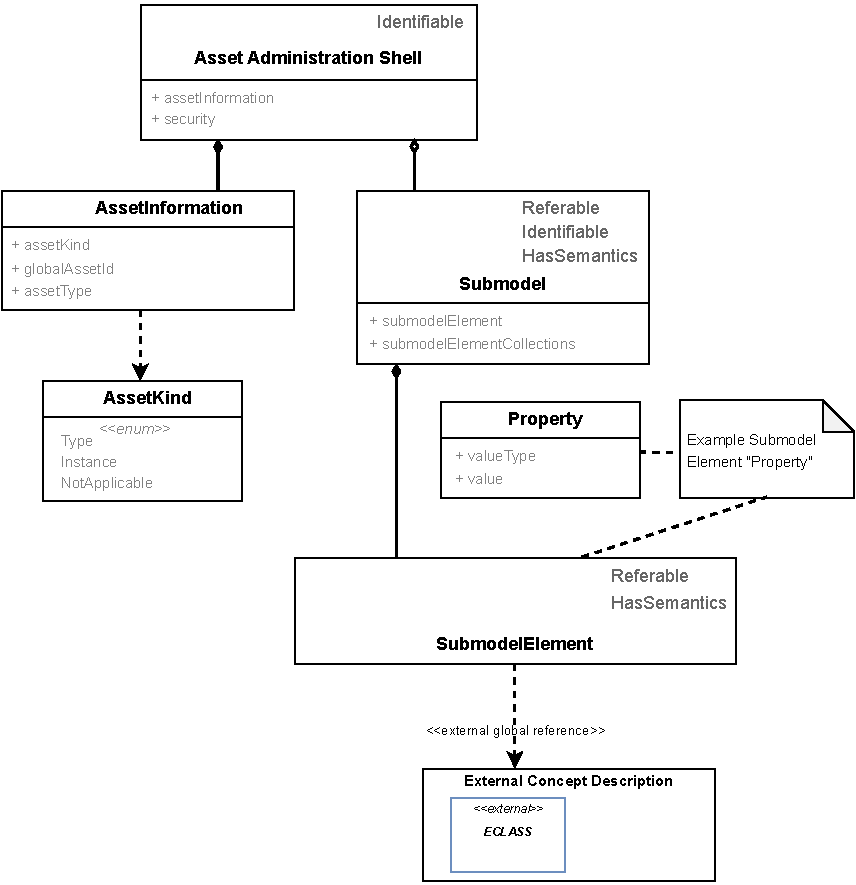
\includegraphics[width=0.9\textwidth]{Bilder/Metamodell_neu.drawio.pdf}
    \caption{Vereinfachtes Metamodell der \acs{aas}}
    \label{fig:MetamodellAAS}
\end{figure}

Wichtig ist, sowohl die AAS selbst als auch ihre Submodelle müssen global eindeutig identifizierbar sein.
Dies wird durch die Verwendung von eindeutigen Identifikatoren der Klasse Identifiable wie einer URI (Uniform Resource Identifier) oder IRDI (International Registration Data Identifier) sichergestellt.
Für die Elemente innerhalb eines Submodells ist eine lokale Kennung ausreichend. Dies erfolgt in der Regel anhand einer idShort der Klasse Referable, die einen kurzen, aussagekräftigen Namen enthält.
Dabei ist wichtig alle Submodelle bzw. alle Elemente über eine eindeutige Semantik zu beschreiben.
Hierfür gibt es eine sogenannte SemanticID der Klasse HasSemantics, welche eine semantische Referenz enthält.
Sie können entweder auf externe Standards oder direkt auf eine Beschreibung innerhalb der \acs{aas}, sogenannte Concept Descriptions, verweisen.
Ein häufig verwendeter externer Standard ist zum Beispiel ECLASS, welcher auf der Norm IEC 61360 \cite{ECLASSIEC61360} basiert.
Darin wird eine standardisierte Struktur für Merkmale und ihre semantische Beschreibungen definiert.
Die Semantik enthält unter anderem Beschreibugen, Definitionen, Einheiten und externe Referenzen für bestimmte Submodelle oder Submodellelemente und helfen bei der Klassifizierung dieser.
Dadurch wird ein gemeinsames Verständnis unterschiedlicher Systeme geschaffen.
Fehlt die semantische Beschreibung, so kann es schnell zu Missverständnissen kommen.
Liegt beispielsweise ein einfacher Wert 25 vor, ist ohne weitere Informationen unklar, was gemeint ist. 
Es könnte sich um 25 Euro, 25 Meter oder 25 Grad Celsius handeln.
Erst durch die zugehörige semantische Beschreibung, in der die Einheit und Bedeutung definiert werden, wird der Wert eindeutig interpretierbar. 


Um die Erstellung von Submodellen zu erleichtern und gleichzeitig Interoperabilität zu gewährleisten, stellt die IDTA standardisierte Submodellvorlagen - sogenannte Submodel Templates - zur Verfügung.
Aktuell sind 34 dieser Templates veröffentlicht, viele weitere sind in der Entwicklung oder im Überprüfungsprozess und werden in Zukunft ergänzt.
Die bereits verfügbaren Templates enthalten unteranderem Submodelle wie das digitale Typenschild oder den Carbon Footprint.
Alle Eigenschaften innerhalb dieser Vorlagen werden dabei in Verbindung mit dem ECLASS-Standard einheiltich semantisch beschrieben.
Diese Templates könen über ein zentrales Repository bezogen werden und bilden die Basis für eine interoperable semantische Datenstruktur.

\subsubsection{Informationsaustausch}
Der Austausch von Informationen über die AAS kann auf unterschiedliche Weise erfolgen.
Die einfachste Möglichkeit besteht im Dateiaustausch. Hierfür wurden speziell für die AAS sogenannte AASX-Dateien \cite{SpezifikationPart5} entwickelt, die den einfachen Austausch statischer \acs{aas} (Typ 1) ermöglichen.
Dabei werden sämtliche Daten, Beziehungen, Strukturen sowie zugehörige Dateien der AAS serialisiert und in ein AASX-ZIP-Dateiformat gespeichert. Diese Datei kann anschließend über ein digitales Medium, etwa per E-Mail oder eine Cloud-Plattform, weitergegeben werden. 
Eine Typ 2-\acs{aas} hingegen wird von einer Laufzeitumgebung gehosted, wodurch ein direkter und dynamischer Zugriff auf ihre Inhalte ermöglicht wird. 
Die Spezifikitation Part 2: Aplication Programming Interfaces \cite{SpezifikationPart2} beschreibt hierfür nicht nur standardisierte Schnittstellen, sonder auch ein ganzheitliches System für das Verwalten, Bereitstellen und Auffinden der AAS.
Repositories dienen dabei als zentraler Speicherort für die Inhalte einer \acs{aas}, einschließlich ihrer Submodelle und Concept Descriptions.
Die Aufgabe der Verwaltung und Registrierung wird von Registries übernommen.
Sie ermöglichen das systemweite Auffinden von \acs{aas} und stellen sicher, dass diese eindeutig referenzierbar sind.
Ergänzend dazu bieten Discovery-Services eine erweiterte Suchfunktionalität, indem sie Beziehungen verschiedener Entitäten mittels verschiedener Schlüsselwertpaare speichern.
Eine AAS kann so zum Beispiel logisch mit einer Asset-Id verknüpft werden und somit schnell innerhalb komplexer Systeme identifiziert werden.
Der Zugriff auf diese Systeme bzw. ihrer Inhalte wird in Form von Schnittstellen standardisiert, wodurch eine hohe Interoperabilität gewährleistet wird.
Ein besonderer Fokus liegt dabei auf HTTP/REST, welches durch definierte Zugriffsprinzipien strukturiert ist. Diese folgen dabei dem REST-Schema und unterstützen gängige HTTP-Methoden wie GET, POST, PUT oder DELETE.
Die fortschrittlichste Form des Informationsaustausches stellt die Peer-to-peer Kommunikation, bei der I4.0-Komponenten (Typ 3-AAS) eigenständig über die I4.0-Sprache miteinander kommunizieren können.



% über gängige Protokolle wie HTTP/REST, MQTT oder OPC UA.
% Diese erlauben externen Systemen gezielt auf bestimmte Daten innerhalb der AAS oder ihrer Submodelle zuzugreifen.
% Die Spezifikation beschreibt außerdem ein System, das im Wesentlichen aus drei Kernkomponenten besteht: Repositories, Registries und Discovery Services.
% werden drei Kernkomponenten beschrieben, die zusammen ein System für einen interoperablen, standardisierten Zugriff bilden.
% Repositories dienen als Speicherort für die Inhalte einer \acs{aas}, einschließlich ihrer Submodelle und Concept Descriptions.
% Die Aufgabe der Verwaltung und Registrierung wird dabei von zentralen Registries übernommen.
% Sie ermöglichen das systemweite Auffinden von \acs{aas} und stellen sicher, dass diese eindeutig referenzierbar sind.
% Ergänzend dazu biete Discovery-Services eine erweiterte Suchfunktionalität, indem sie Beziehungen verschiedener Entitäten mittels verschiedener Schlüsselpaare speichern.
% Eine AAS kann so zum Beispiel logisch mit einer Asset-Id verknüpft werden und somit schnell innerhalb komplexer Systeme identifiziert werden.
% Der Zugriff auf alle dieser Systeme wird in Form von Schnittstellen standardisiert, wodurch eine hohe Interoperabilität gewährleistet wird.
% Die Schnittstellen folgen dabei dem REST-Schema und unterstützen gängige HTTP-Methoden wie GET, POST, PUT oder DELETE.\\
% Die fortschrittlichste Form des Austauschs ist die Peer-to-peer Kommunikation, bei der I4.0-Komponenten (Typ 3-AAS) eigenständig über die I4.0-Sprache miteinander kommunizieren können.

\subsubsection{Sicherheit}
Gerade wenn Informationen aus der \acs{aas} über die Grenzen des eigenen Unternehmens hinweg bereitgestellt werden, ist es besonders wichtig, dass die enthaltenen Daten geschützt sind. 
Die neueste Spezifikation Part 4: Security \cite{SpezifikationPart4} der \acs{idta} liefert hierfür die technische und konzeptionelle Grundlage.
Sie  beschreibt, wie Zugriffe auf Daten in der \acs{aas} sicher gesteuert werden können, insbesondere in vernetzten Umgebungen wie Datenräumen.
Zum Einsatz kommen dabei neue Dienste wie ein Identity Provider zur Authentifizierung oder ein Policy Service zur Durchsetzung von Richtlinien.
Die Sicherheit wird dabei mit Hilfe eines attributbasierten Zugriffsmodells (Attribute Based Access Control (ABAC)) gewährleistet.
Bei jeder Anfrage auf bestimmte Objekte innerhalb der \acs{aas} wird dabei anhand verschiedener Merkmale (Attribute) geprüft ob ein Zugriff erlaubt ist.
Dazu zählen sogenannte Subjektattribute (also wer die Anfrage stellt), Objektattribute (z.B. welches Submodell, welche Property oder welches Submodellelement betroffen ist), die gewünschte Aktion (z.B. Lesen oder Schreiben) sowie kontextbezogene Bedingungen (z.B. Zeitpunkt der Anfrage oder Zustand des Systems).
Die zur Prüfung notwendigen Informationen liefert in der Regel ein Token, das vom Identity Provider bereitgestellt wird. Die Spezifikation sieht hierfür die Nutzung sogenannter JSON Web Tokens (JWT) vor.
Die Attribute werden schließlich von einem Policy Service mit den dort hinterlegenen Zugriffsrichtlinen abgeglichen und basierend darauf eine Zugriffsentscheidung getroffen.
Ein besonderer Vorteil des ABAC-Modells liegt dabei in seiner hohen Flexibilität. Rollen können ebenfalls als Attribute behandelt werden, wodurch sich auch problemlos rollenbasierte Zugriffskonzepte (RBAC) umsetzen lassen. 

Die beschriebenen Kontrollmechanismen lassen sich nicht nur auf die Inhalte der \acs{aas} selbst, sondern insbesondere auch auf die Schnittstellen von Registries und Repositories anwenden.
So kann beispielsweise sichergestellt werden, das nur authorisierte Systeme Zugriff auf ein bestimmtes Submodell erhalten oder nur bestimmte Nutzergruppen neue \acs{aas}-Instanzen registrieren können.
Diese Sicherheits-Konzepte sind jedoch noch vergleichsweise neu und müssen in der Praxis erst noch weiter erprobt werden.
Erste Referenzimplementierungen liegen zwar bereits häufig schon in Form rollenbasierter Zugriffskontrollen vor, eine vollständige Integration des ABAC-Ansatzes steht jedoch noch aus.


\subsection{Digitaler Produktpass}
Der \ac{dpp} ist ein zentrales Instrument der Europäischen Union zur Umsetzung einer nachhaltigen, digitalen Transformation.
Ziel ist es, die Transparenz über ökologische Merkmale von Produkten wie verwendete Materialien, Recylcebarkeit oder die CO2-Bilanz deutlich zu verbessern.
Hierzu müssen produktspezifische Daten über den gesamten Lebenszyklus hinweg aufgezeichnet und in einem menschen -und maschinenlesbarem Format bereitgestellt werden.
Langfristig soll dies zu einer Kreislaufwirtschaft und digitalen Wirtschaft innerhalb der EU führen.

Das Konzept des digitalen Produktpasse wurde erstmals im Rahmen des European Green Deal von der Europäischen Kommission im Jahr 2019 vorgestellt \cite{GreenDeal}.
Im Zuge der Ökodesign-Verordnugng (Eco Design for Sustainable Products Regulation (ESPR) ) \cite{ESPR} wird der \acs{dpp} aktuell als verpflichtendes Mittel für zahlreiche Produktgruppen eingeführt.
Als erstes konkrete Anwendung wird der digitale Produktpass erstmals im Jahr 2027 für Batterien verpflichtend, wie in der EU-Batterieverordnung festgelegt.
Weitere Produktkategorien, darunter auch die Elektroindustrie und der Maschinen -und Anlagenbau werden in den nächsten Jahren folgen.

Die Bereitstellung der digitalen Produktpässe erfolgt gemäß den Anforderungen der ESPR in elektronischer Form. Dabei müssen diese untereinander interoperabel miteinander kommunizieren können.
Daten innerhalb eines Passes müssen standardisiert und strukturiert in einem menschen -und maschinenlesbarem Format zur Verfügung gestellt werden.
Je nach Art der Information werden verschiedene Zugriffsrechte für unterschiedliche Interessengruppen eingeführt. Damit soll der Schutz von geistigem Eigentum sichergestellt werden.
Verwaltet werden sollen die Daten dabei über einen zentralen Server bzw. ein Registry, in dem die verschiedenen \acsp{dpp} gespeichert bzw. zumindest registriert werden.
Der Zugriff auf konkrete Pässe soll möglichst einfach sein. Hierzu können zum Beispiel QR-Codes eingesetzte werden, die direkt am Produkt angebracht sind, und direkt zum \acs{dpp} führen.
Dafür ist es wichtig, das jedes Produkt global eindeutig über eine einzigartige Kennung beschrieben wird.
\cite{CIRPASS}

Während die regulatorischen Rahmenbedingungen schon mehr oder weniger final ausgearbeitet sind, bleibt noch die Frage der konkreten technologischen Umsetzung.
Eine dezentrale Lösung zur Umsetzung bildet der von der ZVEI vorgestellte digitale Produktpass für die Industrie 4.0 (DPP 4.0) \cite{DPP40}.
Der DPP 4.0 basiert dabei auf zwei etablierten Standards. Zum Einen das digitale Typenschild, und zum Anderen die AAS (siehe auch Kapitel~\nameref{chap:AAS}).
Das digitale Typenschild ermöglicht - gemäß der Norm IEC 61406 \cite{TypenschildIEC61406-1} - die eindeutige Identifikation von Produkten über eine einzigartige Asset-ID.
Typischerweise wird diese in Form eines maschinenlesbarem Links oder QR-Codes an ein Produkt angebracht, wodurch ein direkter Zugriff auf den jeweiligen \acs{dpp} ermöglicht wird.

Organisiert werden die Daten im DPP 4.0 in verschiedenen Submodellen der AAS. 
Standardisierte Teilmodelle wie das digitale Typenschild, Dokumentationen oder der Product Carbon Footprint (PCF) helfen bei der Umsetzung der im \acs{dpp} geforderten Daten.
Darüber hinaus können auch zusätzliche, nicht verpflichtende Informationen integrierte werden, sofern sie für bestimmte Stakeholder einen Mehrwert bieten.
Der Zugriff auf die Daten erfolgt über ein webbasiertes Portal. Verschiedene Interessengruppen erhalten dabei unterschiedliche Zugangsrechte. 
Hierfür werden bestimmmte Submodelle gezielt für unterschiedliche Gruppen freigegeben oder eingeschränkt.
Während beispielsweise das digitale Typenschild (DN) oder der PCF öffentlich zugänglich sind, werden sensible Informationen wie technische Dokumentationen oder sicherheitsrelevante Details nur bestimmten autorisierten Gruppen zugänglich gemacht.
Eine schemantische Darstellung des DPP 4.0 ist nachfolgend in Abbildung xy dargestellt.

\vspace{1em}
\begin{figure}[htbp]
    \centering
    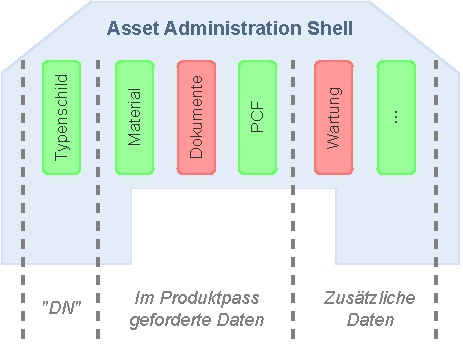
\includegraphics[width=0.7\textwidth]{Bilder/dpp_konzept.pdf}
    \caption{Konzept des DPP 4.0}
    \label{fig:klassifizierungDT}
\end{figure}

Das Konzept der ZVEI sieht darüber hinaus vor, dass Unternehmen ihre digitalen Produktpässe etgegen den Anforderungen der ESPR dezentral in einem eigenen Repository verwalten. 
Diese Repositories können entweder vom produzierenden Unternehmen selbst oder von Dritten - etwa Cloud-Dienstleistern - im Auftrag betrieben werden. 
Ziel ist es, Unternehmen die Möglichkeit zu geben, ihre Daten bei Bedarf eigenständig zu aktualisieren und gleichzeitig die Kontrolle über sensible Informationen zu behalten.
Zur Koordination dieser dezentralen Systeme ist ein zentrales Registry vorgesehen, in der alle Repositories bzw. Server registriert werden.
Über dieses zentrale Verzeichnis können interessierte Akteure relevante Server identifizieren und gezielt auf freigegebene Submodelle eines Produktpasses zugreifen.
So wird sichergestellt, dass trotz der dezentralen Struktur eine durchgängige Interoperabilität gewährleistet ist, wie sie für die Umsetzung des digitalen Produktpasses auf europäischer Ebene erforderlich ist.

%

\subsection{robocell Füll -und Verschließmodul}
Die robocell ist eine von groninger in Zusammenarbeit mit SKAN entwickelte Maschinenlinie zur Abfüllung von Spritzen, Vials und ....
Sie zeichnet sich dadurch aus, das das Abfüllen voll automatisiert ist. Durch den Einsatz von Robotern entlang des gesamten Abfüllprozesses, entfällt somit die Notwendigkeit eines menschlichen Eingriffes.
Die Linie besteht dabei aus verschiedenen Modulen.
Diese einzelknen Maschinen sind dafür speziell für eine bestimmte Aufgabe entlang des Prozesses verantwortlich.
Dies geht von der automatisierten Entpackung von den abzufüllenden Behältern über das Füllen bis hin zur automatisierten Verpackung der Behältnisse.
Im Abfüll -und Verschließmodul werden die Behälter zuerst mit Hilfe einer Schlauchpumpe gefüllt. Anhscließend werden die Behältnisse mit einem Roboter weitergegeben und mit Hilfe eines Kamerasystrems die Stopfen gesetzt.
Was ist die robocell? Wodurch zeichnet sie sich aus?

Eingehen auf das Füllmodul


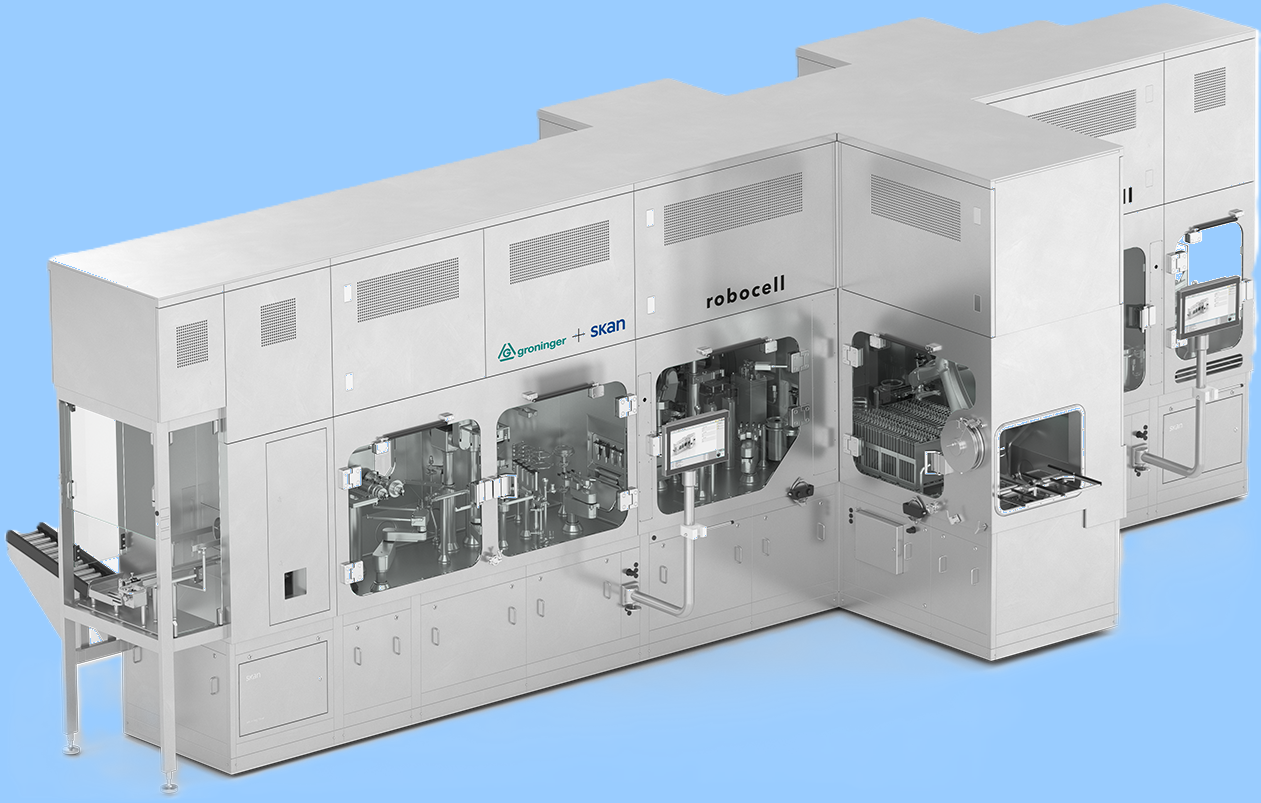
\includegraphics{Bilder/robocell_FS2_rgb_Logo.png}
\subsection{Technologische Grundlagen}
\newpage
\subsubsection{AASX Package Exlporer}
Der AASX Package Explorer wurde als Referenzimplementierung für die AAS gemäß den Spezifikationen der \acs{idta} entwickelt.
Das Tool ist als Open-Source-Software \cite{AASXPackageExplorer} verfügbar und ermöglicht das Erstellen und Bearbeiten von \acs{aas} im standardisierten AASX-Dateiformat.
Er verfügt über eine benutzerfreundliche grafische Oberfläche (siehe Abbildung \ref{fig:AASXPackageExplorer}), die insbesondere Einsteigern den Zugang zur Modellierung erleichtert.
Gleichzeitig bietet der AASX Package Explorer auch erweiterte Funktionen, wie das Erstellen von Submodell-Templates, wodurch er sich auch für den profesionellen Einsatz eignet.

\begin{figure}[htbp]
    \centering
    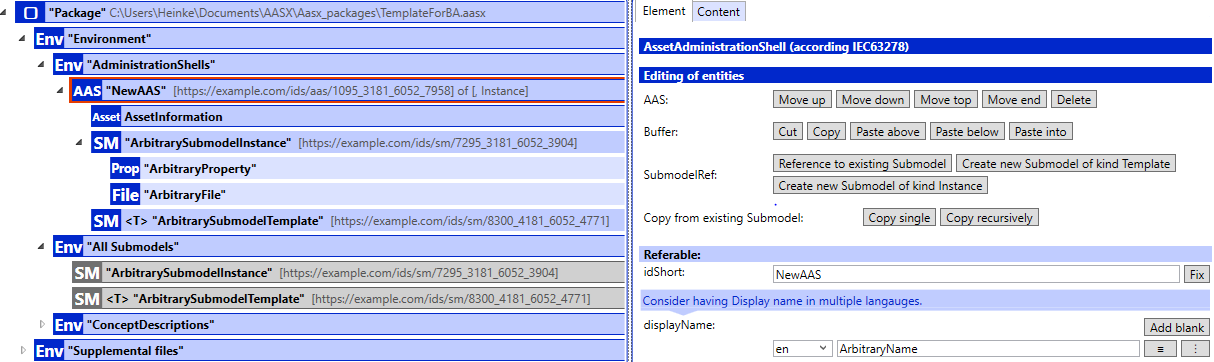
\includegraphics[width=1\textwidth]{Bilder/AAS_PE.PNG}
    \caption{Benutzeroberfläche AASX Package Explorer}
    \label{fig:AASXPackageExplorer}
\end{figure}






% Er ermöglicht das Modellieren von Verwaltungsschalen mit allen Elementen dieser.
% Hiermit können ganze Verwaltungsschale erstellt werden und in eine Datei wie eine aasx Datei oder XML Datei geschrieben werden.
% Er bringt alles mit, was für die Erstellung von Verwaltungsschalen benötigt wird.
% Man kann AAS anschauen und bearbeiten.
% AUch kann ein Server angebunden werden.
\newpage
\subsubsection{Eclipse BaSyx }
Eclipse BaSyx ist eine vom Fraunhofer-Institut für Experimentelles Software Engineering entwickelte Open-Source-Plattform für die Realisierung von Industrie 4.0 - Anwendungen.
Der Fokus liegt auf einer einfachen Umsetzung einer Infrastruktur zur Erstellung und Verwaltung digitaler Zwillinge auf Basis der \acs{aas}.
Ein wesentlicher Vorteil von BaSyx ist sein Open-Source-Charakter. Die Software steht allen Interessierten frei zur Verfügung und erlaubt individuelle Modifikationen an spezifische Anforderungen.
Die Architektur basiert auf einer Vielzahl von Standardkomponenten (Off-the-Shelf), die alle als Docker-Container frei zugänglich sind und somit eine nahtlose Integration in bestehende Docker-Umgebungen erlauben.

Eine der wichtigsten Komponenten ist die Registry. 
Sie ist auf den Spezifikationen der Verwaltungsschale aufgebaut, insbesondere auf der Spezifikation Part 2: Application Programming Interfaces \cite{SpezifikationPart2}.
In ihr können neue \acs{aas} registriert und bereits vorhandene Verwaltungsschalen anhand ihrer eindeutigen Kennung gesucht werden.
Sie bildet damit die zentrale Anlaufstelle für Geräte und Anwendungen innerhalb eines Industrie-4.0-Systems
Analog dazu gibt es eine seperate Registry für die Verwaltung von Submodellen.

Die eigentlichen Daten der AAS werden in der sogenannten \acs{aas} Environment gespeichert und organisiert.
Sie umfasst Repositories für AAS, Submodelle und Concept Descriptions.
In der Regel ist eine Datenbank, standardmäßig eine MongoDB als persistenter Speicher hinterlegt.
Wie auch alle anderen Komponente stellen diese Repositories standardisierte Schnittstellen basierend auf der API-Spezifikation zur Verfügung.
Dies erlaubt z.B. das Abfragen, Erstellen oder Aktualisieren von AAS und deren Submodellen.
Alle verfügbaren Endpunkte dieser Schnittstellen können unter anderem in der automatisch generierten Swagger-Dokumentation eingesehen und ausgeführt werden. 
Typische REST-Endpunkte sind beispielsweise:

\vspace{1em}
\begin{table}[htbp]
    \centering
    \begin{tabular}{l l l}
        \toprule
        \textbf{Methode} & \textbf{Endpunkt} & \textbf{Beschreibung} \\
        \toprule
        \textbf{\textcolor{green!50!black}{\textit{GET}}}     & \texttt{\textit{/shells}} & Liste aller AAS abrufen \\
        \textbf{\textcolor{green!50!black}{\textit{GET}}}     & \texttt{\textit{/shells/\{aasIdentifier\}}} & Bestimmte AAS anzeigen \\
        \textbf{\textcolor{green!50!black}{\textit{GET}}}     & \texttt{\textit{/submodels}} & Liste aller Submodelle aufrufen \\
        \textbf{\textcolor{orange!85!black}{\textit{POST}}}    & \texttt{\textit{/shells}} & Neue AAS erstellen \\
        \textbf{\textcolor{orange!85!black}{\textit{POST}}}    & \texttt{\textit{/submodels}} & Neues Submodell erstellen \\
        \textbf{\textcolor{red!80!black}{\textit{DELETE}}}  & \texttt{\textit{/shells/\{aasIdentifier\}}} & AAS löschen \\
        \midrule
    \end{tabular}
    \caption{REST-Endpunkte in Eclipse BaSyx}
    \label{tab:aas_endpoints}
\end{table}

Im BaSyx-System ermöglicht sin sogenannter Discovery-Service die Verknüpfung physischer Assets mit iheren zugehörigen AAS.
Dabei wird eine spezifische Asset-Id mit der entsprechenden AAS-ID verlinkt.
Dies ist insbesondere für die Abbildung von hierarchischen Strukturen wie Stücklisten (Bill of Materials, BOM) von großer Bedeutung.
Ein übergeordnetes Asset (z.B. Maschine) kann so beispielsweise mit untergeordneten Komponenten (z.B. Antrieb, Sensoren) logisch über deren AAS verbunden werden.
Einträge in den Discovery-Service müssen derzeit allerdings noch manuell über die API vorgenommen werden.

Zur benutzerfreundlichen Visualisierung und Interaktion kann die sogenannte AAS Web Ui genutzt werden.
Die webbasierte Benutzeroberfläche wurde mit dem JavaScript-Framework Vue.js entwickelt und kommuniziert über die standardisierte REST-API mit den zentralen Komponenten der BaSyx-Plattform, darunter die Repositories, Registries und der Discovery Service.
Sie zeigt alle registrierten AAS in einer Liste an und bietet die Möglichkeit, einzelne AAS in einer Baumstruktur sowohl zu visualisieren als auch zu bearbeiten. 
Darüber hinaus unterstützt die Anwendung das Hochladen von Typ-1-AAS in Form von AASX-Dateien. Diese werden automatisch registriert und in eine Typ-2-AAS überführt, wodurch sie direkt in das System eingebunden werden können.
Ein weiteres zentrales Merkmal der AAS Web UI ist der sogenannte AAS-Viewer.
Dieser erlaubt die Visualisierung von Submodellen und deren Elementen anhand ihrer semantischen ID. 
Hierfür stehen verschiedene vordefinierte Plugins zur Verfügung, die bestimmte Submodelle - wie beispielsweise das Typenschild oder hierarchische Strukturen - grafisch darstellen.
Da die Lösung Open Source ist besteht zudem die Möglichkeit, eigene benutzerdefinierte Plugins für weitere Submodelle zu erstellen. \cite{BaSyxWiki} \cite{BaSyxEclipse}

\subsubsection{OPC UA}